\chapter{Elaboration of the Workflow}
\label{chap:elaboration-of-the-workflow}

In this chapter I demonstrate the various steps of the workflow in detail. I introduce small working source code examples and show, how the given step transforms it.

\section{Transforming the Source Code Into an AST}
As mentioned in~\Cref{sect:overview-transforming-the-source-code}, this transformation is carried out by the Shape Security Shift toolkit. The parser is given the source code and the top-level non-terminal it should consider the root of the tree. Considering the new constructs introduced in ES6, I've chosen \emph{Module} as the type of the root.

The only one line long source code in~\Cref{lst:oneliner} parsed and serialized as a tree can be seen in~\Cref{lst:oneliner-ast-json}.

\begin{figure}[!htb]
	\begin{minipage}{\textwidth}
		\lstinputlisting[
			language=JavaScript,
			captionpos=b,
			caption={Basic example source code.},
			label={lst:oneliner},
		]{include/sources/oneliner.js}
	\end{minipage}
\end{figure}

\begin{figure}[!htb]
	\begin{minipage}{\textwidth}
		\lstinputlisting[
			language=JSON,
			captionpos=b,
			caption={AST output of the parser serialized in JSON format.},
			label={lst:oneliner-ast-json},
		]{include/sources/oneliner-ast.json}
	\end{minipage}
\end{figure}

\section{Storing the ASG in the Graph Database}

\section{Division by Zero}
As one of the most basic and easy-to-discover mistakes, division by zero should be reported to the developer. In the context of mathematics, division by zero is undefined for the real numbers. In JavaScript, it may result in \code{NaN} or \code{Infinity}.

Without dynamic testing or symbolic execution it is rather hard to find this kind of expression, since the right side of the division may come from a variable. On the other hand, finding the cases where the right side is a literal is trivial.

Taking a look at the graph representation of the previous example (in~\Cref{fig:AST-PPT}), it is relatively easy to find the problematic nodes. A natural language definition of the problem would sound like: ,,we are looking for binary expressions that have a literal zero on the right side''.

\begin{figure}[!htb]
  \centering
  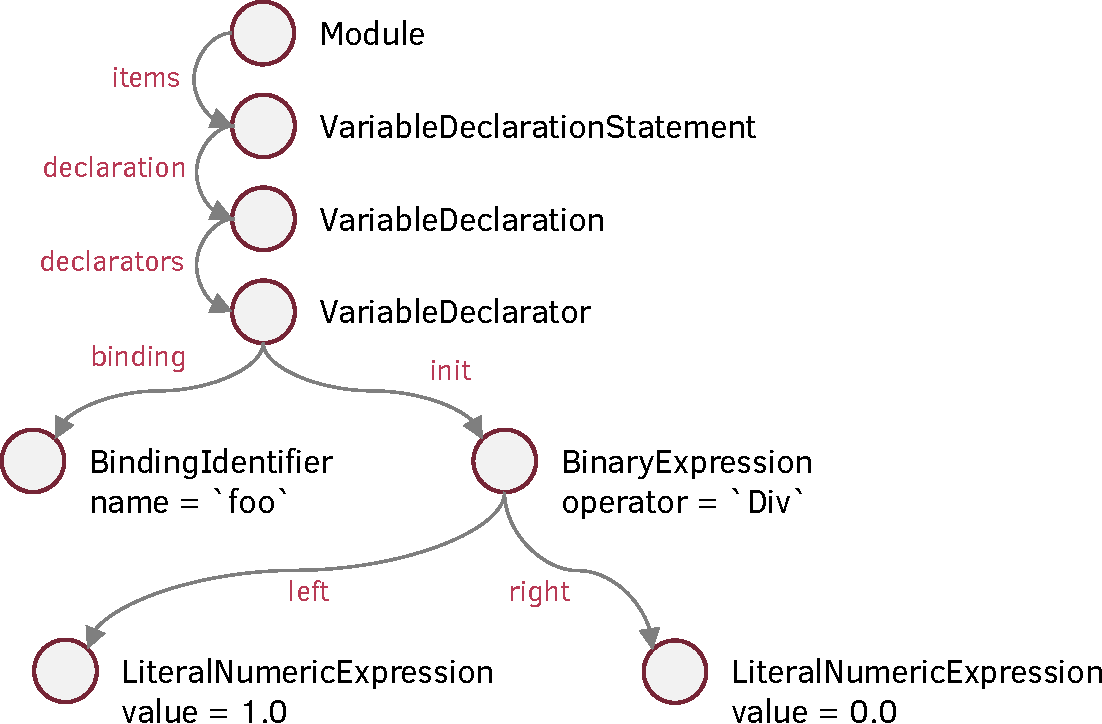
\includegraphics[width=0.8\textwidth]{AST-PPT.pdf}
  \caption{Graph Representation of the One Line Long Source Code}
  \label{fig:AST-PPT}
\end{figure}

One way to formalize this declarative definition in Cypher can be seen in~\Cref{lst:division-by-zero}. Executing this query would find matching nodes with the right type, bind them to the corresponding names and check, whether the required relations are present, resulting in a state like in~\Cref{fig:AST-query-PPT}. Finally the result is the \code{BinaryExpression} node that can be used to get the precise location of the expression in the source code and report it as problematic.

\begin{figure}[!htb]
	\begin{minipage}{\textwidth}
		\lstinputlisting[
			language=Cypher,
			captionpos=b,
			caption={Graph Pattern Matching Division by Zero.},
			label={lst:division-by-zero}
		]{include/sources/division-by-zero.cypher}
	\end{minipage}
\end{figure}

\begin{figure}[!htb]
  \centering
  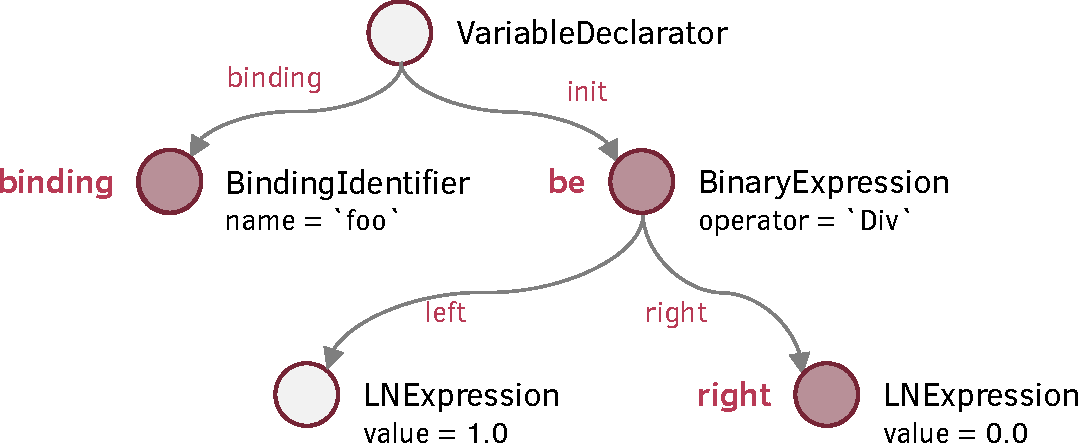
\includegraphics[width=0.8\textwidth]{AST-query-PPT.pdf}
  \caption{Graph Representation of the Query Searching Division by Zero}
  \label{fig:AST-query-PPT}
\end{figure}

\section{Handling Import and Export}
Since the beginning, JavaScript projects have grown tremendously. With the size of the average project, the language has also matured for handling bigger, more complex code repositories. With ES6, a module syntax has been introduced to spread the codebase into files, even directories. (Even before ES6 there have been several module systems, but ES6 described a standard for it.)

As I've mentioned before, I instruct the parser to process source files as modules. An ES6 \emph{module} differs in two ways from a \emph{script}: it is automatically interpreted as a \emph{strict-mode code}, and one can use \code{import} and \code{export} statements in them.

This section follows
% TODO https://hacks.mozilla.org/2015/08/es6-in-depth-modules/
% TODO https://developer.mozilla.org/en-US/docs/Web/JavaScript/Reference/Statements/import
% TODO https://developer.mozilla.org/en-US/docs/Web/JavaScript/Reference/Statements/export
and collects the most important details about the specifications.


\subsection{Export}
Everything declared inside a module belongs to the scope of the module. In order to let other modules to access them, they need to be explicitly exported.

\Cref{lst:es6-export} lists the various ways declaring a feature export. Just to list a few combinations; one may, for example, export expressions, variables, function and generator declaration statements either named, or using an alias. Or have default export expressions, even in an export statement.

\begin{figure}[htbp]
	\begin{minipage}{\textwidth}
		\lstinputlisting[
			language=JavaScript,
			captionpos=b,
			caption={ES6 Export Statement Examples from MDN.},
			label={lst:es6-export},
		]{include/sources/es6-export-mdn.js}
	\end{minipage}
\end{figure}

Parsing these export statements result in different representation in the instance model and the resulting graph. \Cref{fig:es6-export-example} shows an example inline default export statement for a function named \code{foo}: \code{export default function foo() \{\}}. Note that the export statements are listed in the \code{Module}, but not in any of the \code{Scope}s.

\begin{figure}[htbp]
  \centering
  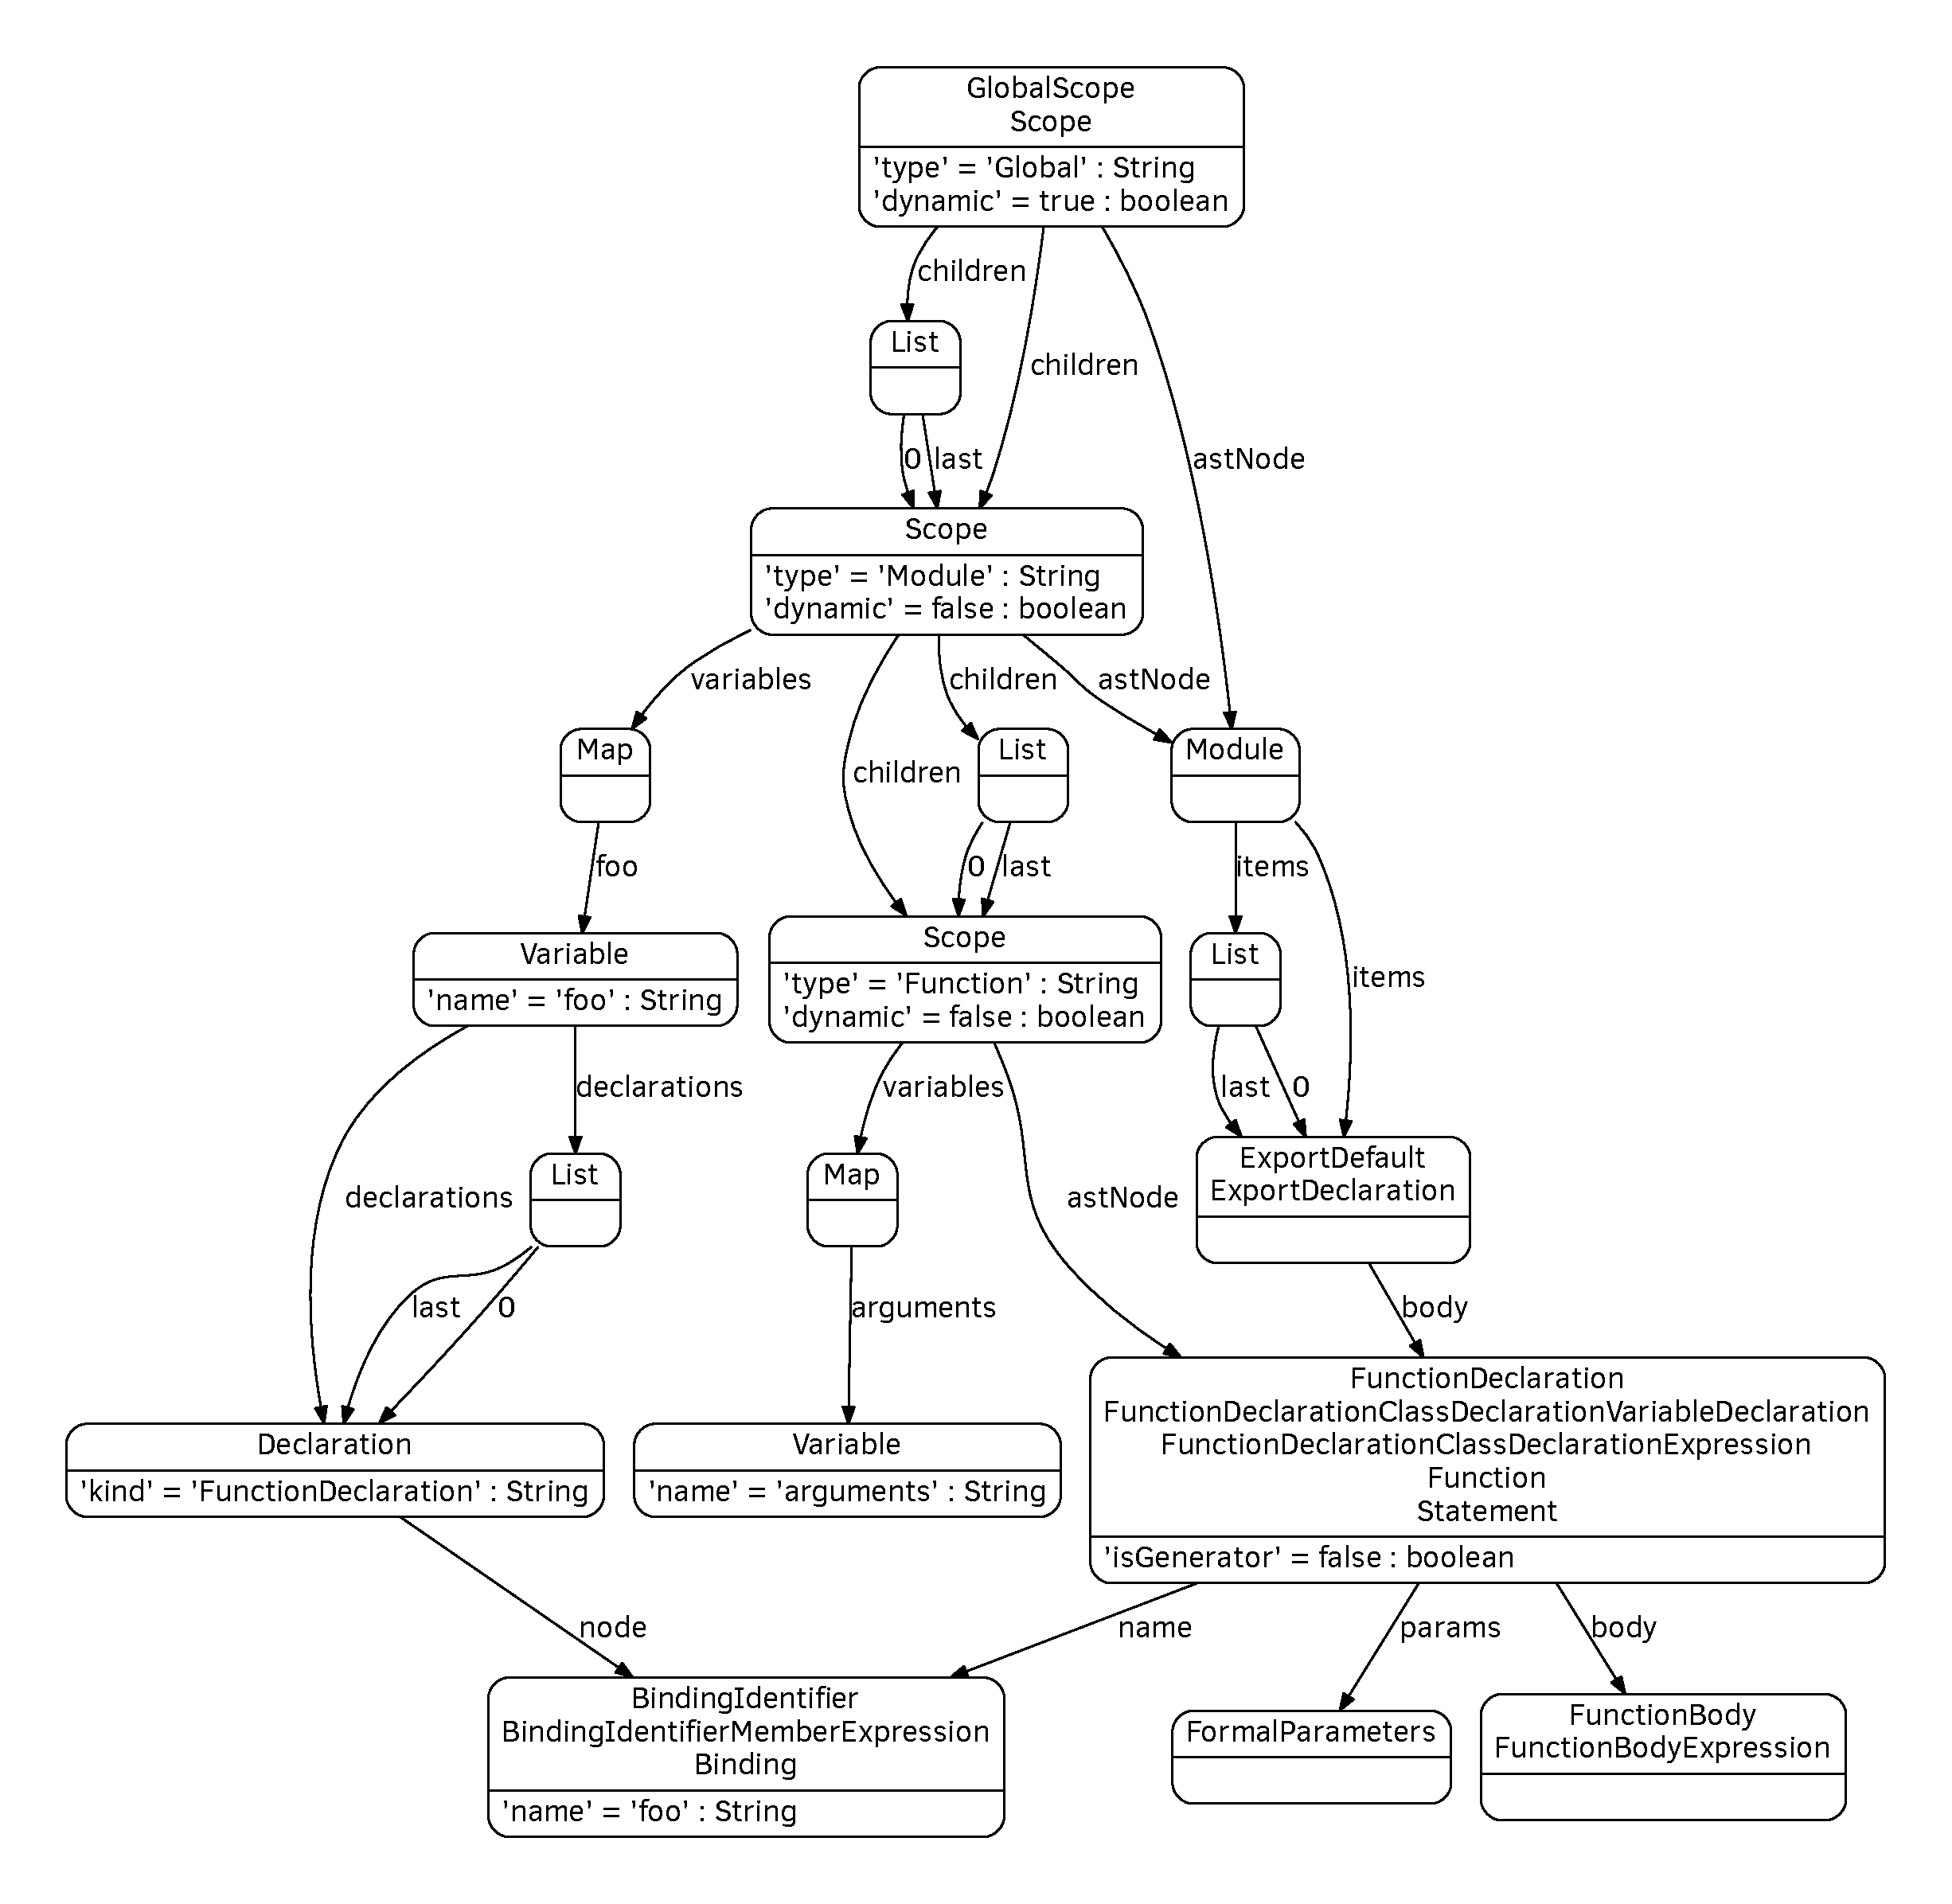
\includegraphics[width=0.8\textwidth]{export-example}
  \caption{ES6 Export Statement Example}
  \label{fig:es6-export-example}
\end{figure}


\subsection{Import}
Like there are many ways for exporting features in a module, there are also several ways for importing them. \Cref{lst:es6-import} lists these.

\begin{figure}[htbp]
	\begin{minipage}{\textwidth}
		\lstinputlisting[
			language=JavaScript,
			captionpos=b,
			caption={ES6 Import Statement Examples from MDN.},
			label={lst:es6-import},
		]{include/sources/es6-import-mdn.js}
	\end{minipage}
\end{figure}

The imported features are placed in the module-level global scope as a \code{Variable} without their declaring node, and the import statements are also present in the AST. \Cref{fig:es6-import-example} shows the ASG of a module importing and then using a function declaration (exported in the previous module): \code{import foo from "export"; foo();}.

\begin{figure}[htbp]
  \centering
  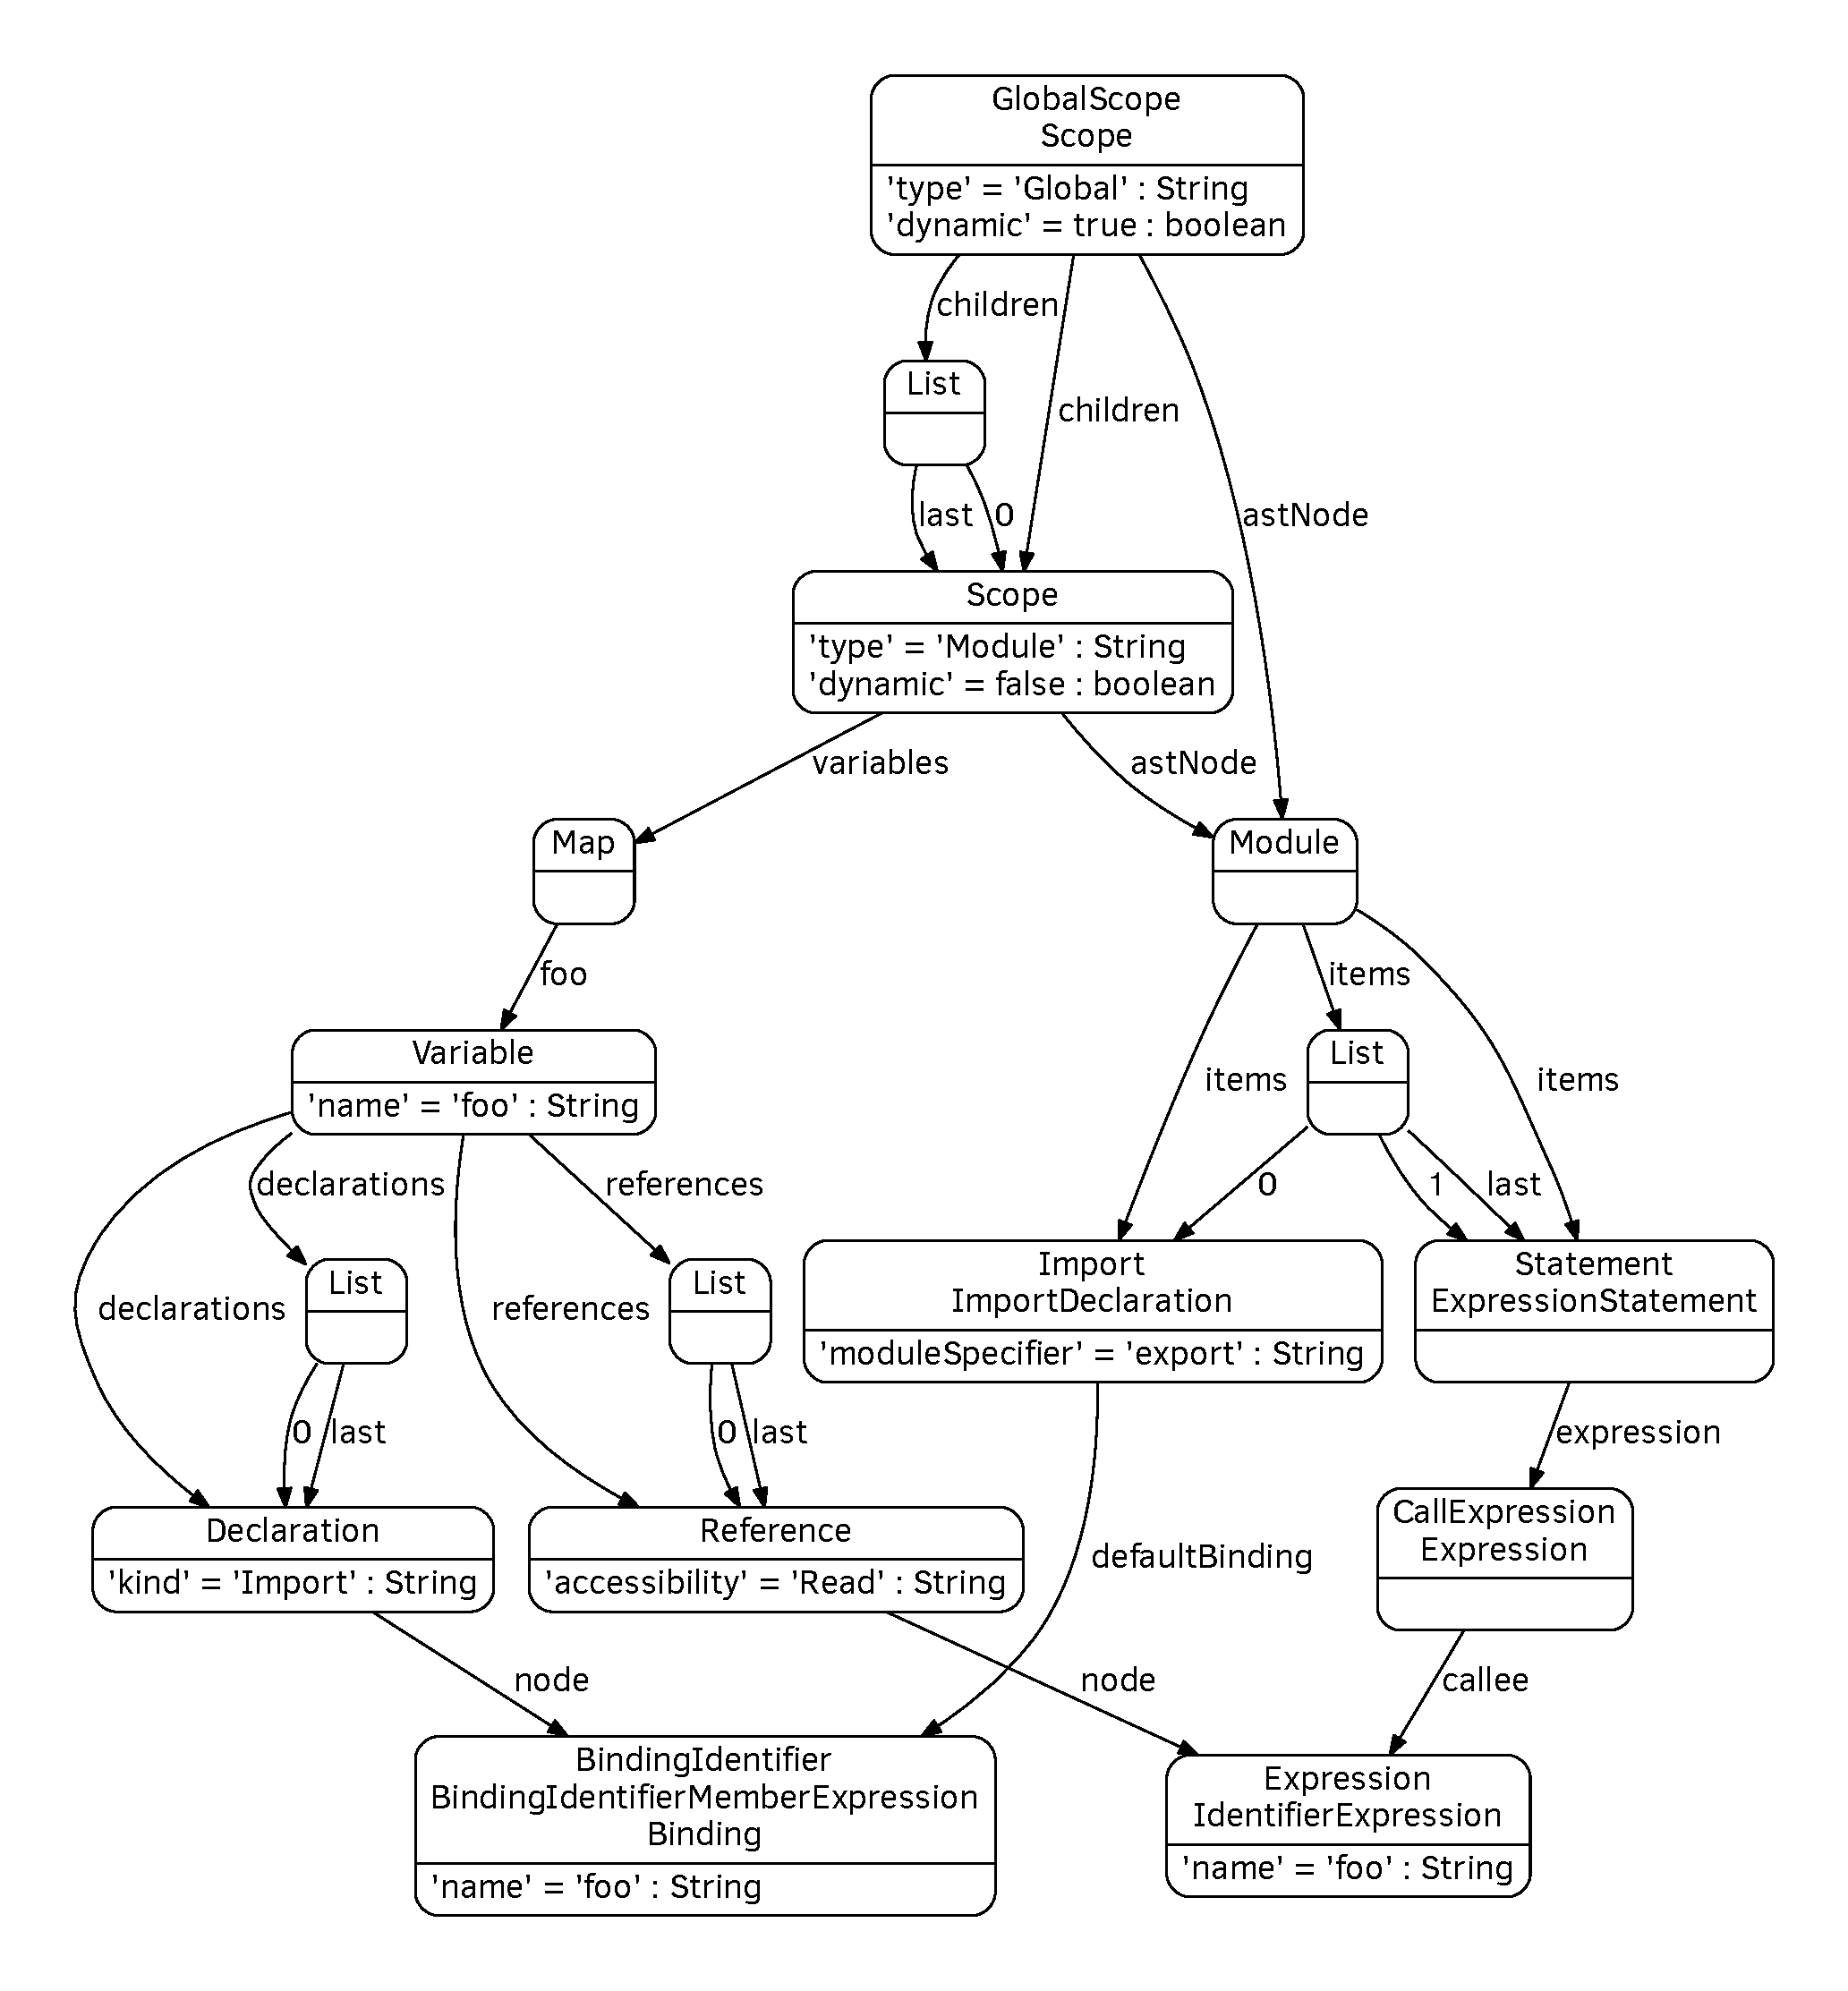
\includegraphics[width=0.8\textwidth]{import-example}
  \caption{ES6 Import Statement Example}
  \label{fig:es6-import-example}
\end{figure}


\subsection{Connecting Imports to Exports}
Since there are several ways to export and import features, there are even more combinations of these. This paper does not aim to cover all of these, but to show that it's possible to connect graph module representations based.

Executing the following steps emulates the resolution made by the interpreter of the source codes and connects the usages of the imported feature to the declaration of the exported one:

\begin{enumerate}[topsep=0pt]
	\item Find the imported \code{IdentifierExporession} in the \code{items} list of the \code{GlobalScope} node.
	\item Find the connected upstream \code{Variable} node.
	\item Find the \code{Declaration} for the \code{Export} that has a \code{Node} with the same \code{BindingIdentifier} as the import.
	\item Connect the \code{Variable} on the import side to the \code{Declaration} on the export side with a \code{declarations} relation.
\end{enumerate}

The Cypher query in~\Cref{lst:connect-import-export} manages to connect the exact type of imports and exports mentioned in the previous sections. Note that this query does not search for a file exporting the statement. For the correct match it should also check the metadata, whether the found node was declared in a file with matching absolute path.
% TODO absolute path

\begin{figure}[!htb]
	\begin{minipage}{\textwidth}
		\lstinputlisting[
			language=Cypher,
			captionpos=b,
			caption={Cypher Query for Connecting Import and Export Statements.},
			label={lst:connect-import-export}
		]{include/sources/connect-import-export.cypher}
	\end{minipage}
\end{figure}

After executing the query in~\Cref{lst:connect-import-export}, the two ASG subgraphs are connected with a new edge (see~\Cref{fig:import-export-example}). This makes it possible to execute global-level queries addressing multiple modules. These newly added relations are always removed when either the source or the destination is removed, in case a module is modified. Thus it is optimal to run this query only when all of the files are already processed and the chance of modification in the near future is low.

\begin{sidewaysfigure}[htbp]
  \centering
  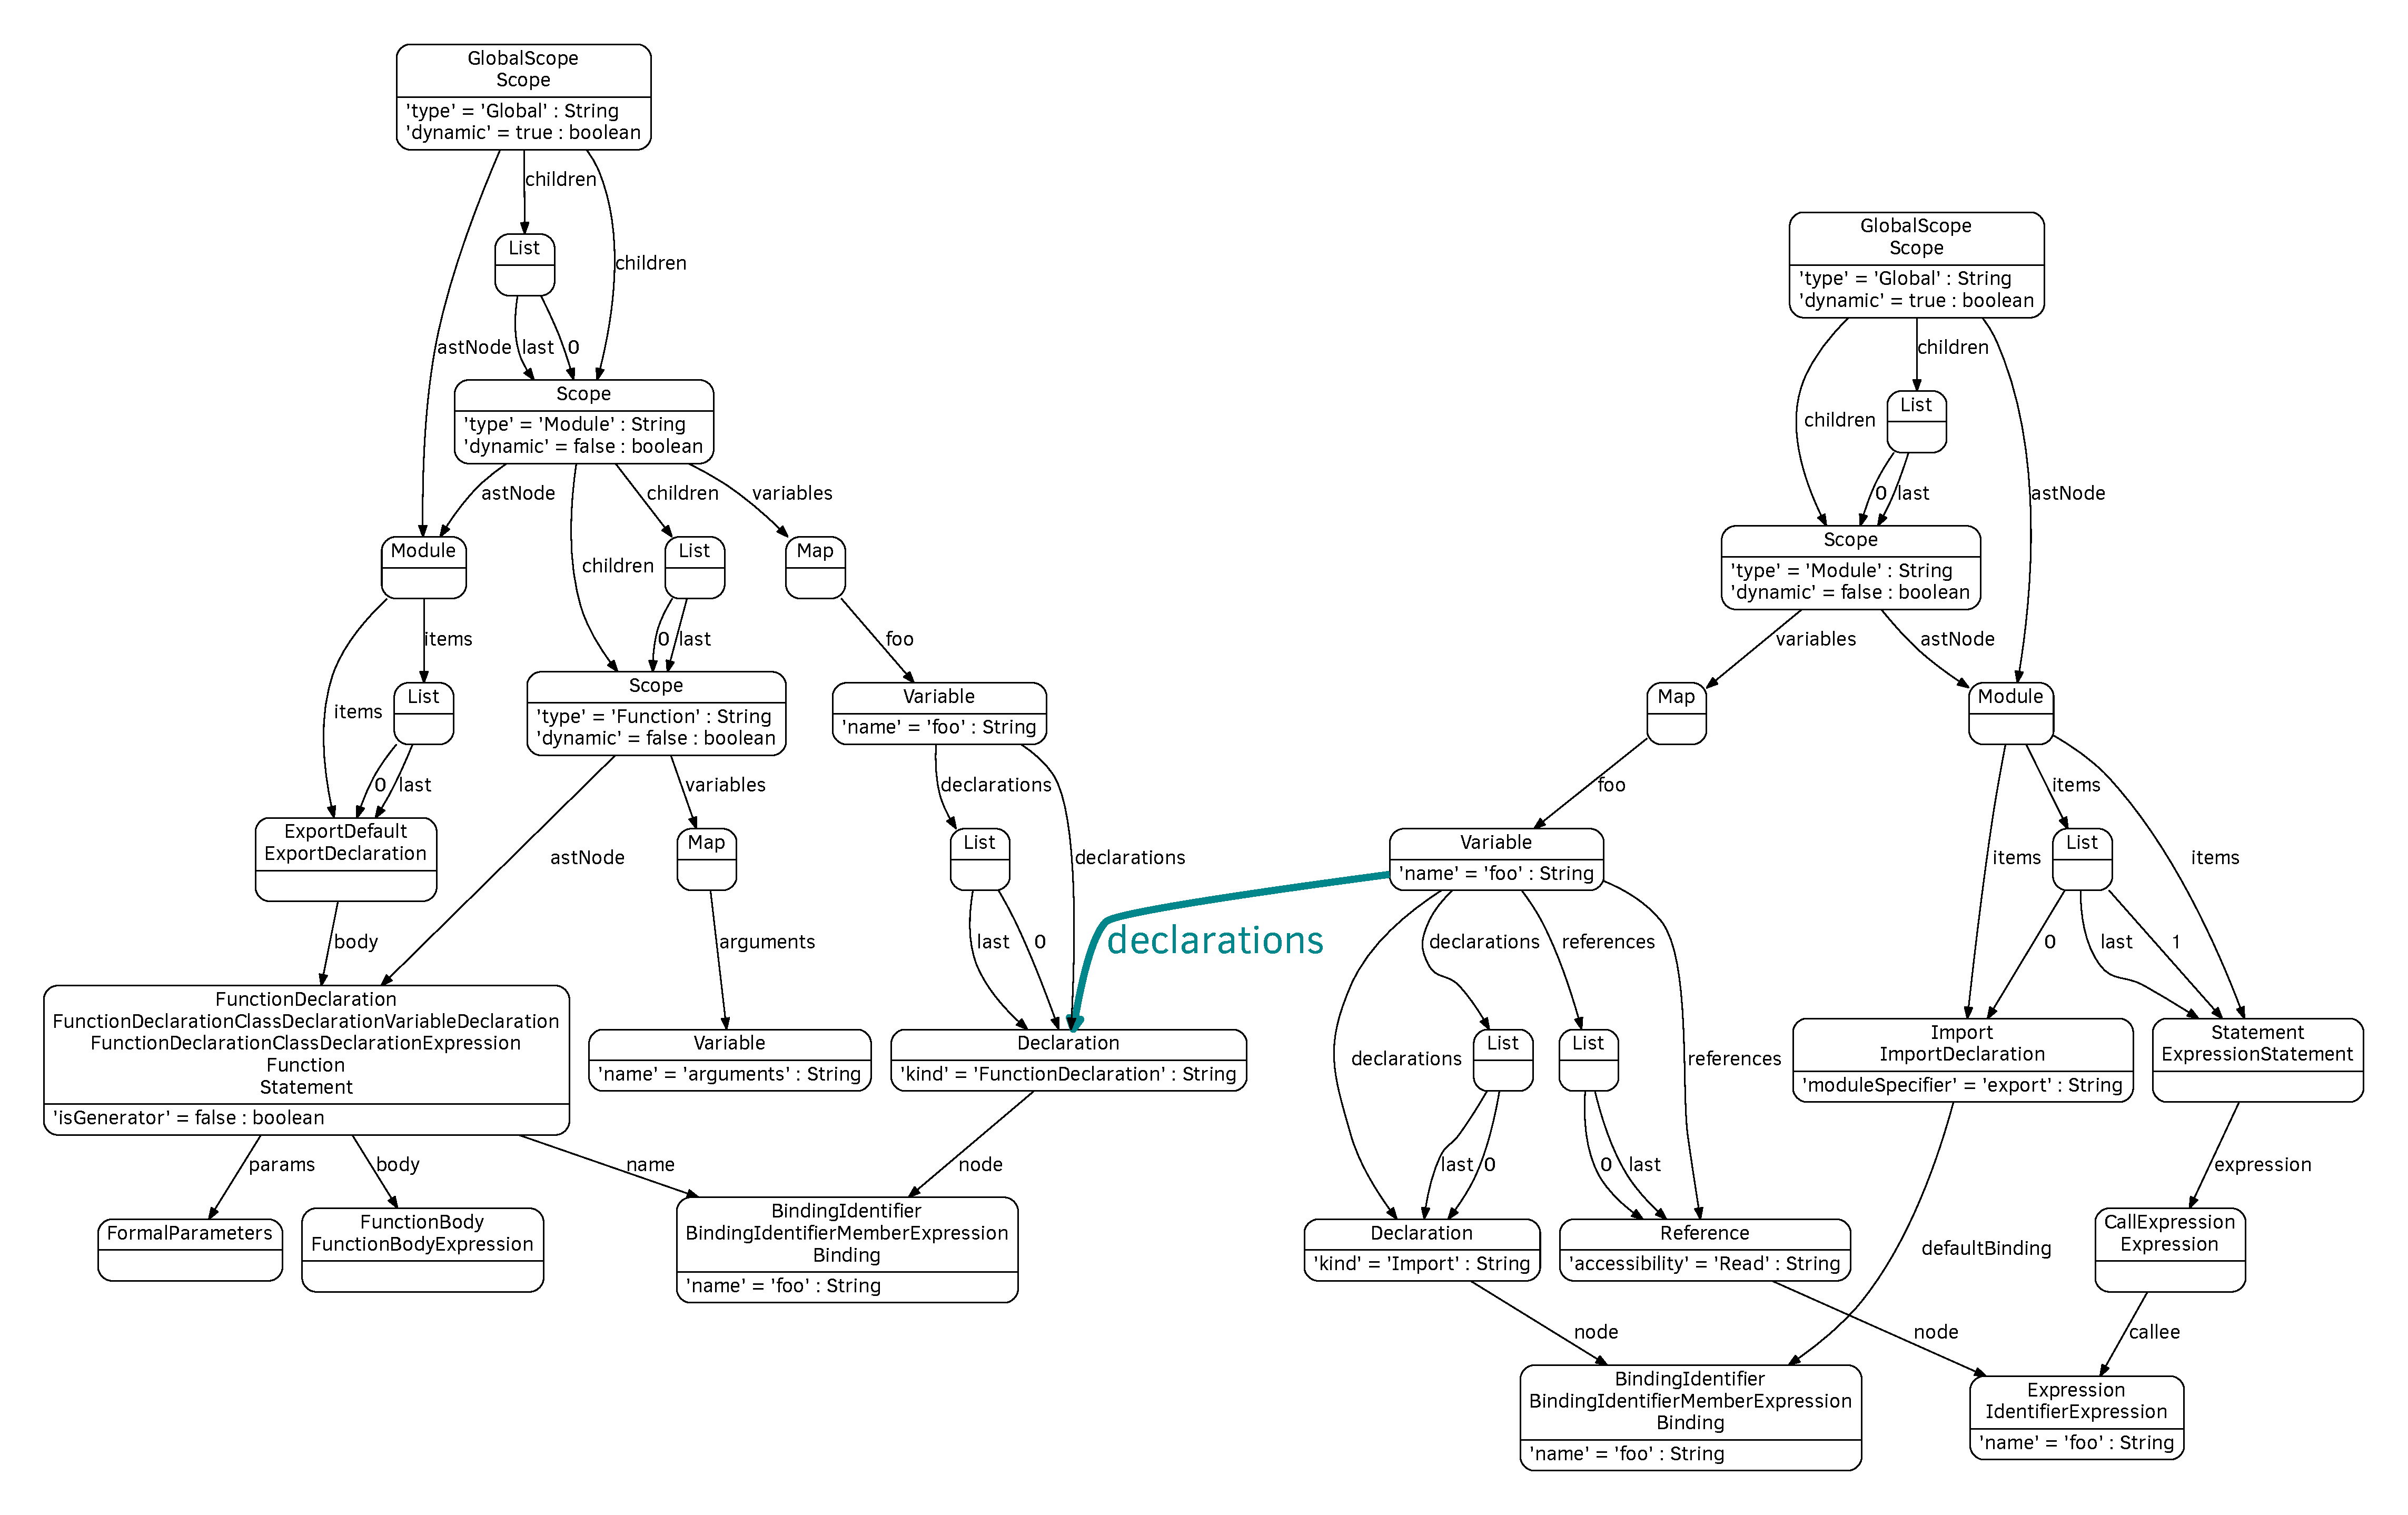
\includegraphics[width=\textwidth]{import-export-example}
  \caption{Merged ASG Subgraphs}
  \label{fig:import-export-example}
\end{sidewaysfigure}


\section{Dead Code Search}
Code that is written, but not used in the whole codebase is often called \emph{dead code}. Without symbolic execution or dynamic analysis it is not possible to decide what part of the code is reachable, but (excluding dynamic evaluation --- eg., \code{eval} in JavaScript) it is feasible to find function declarations in a file that are possibly not referenced in the local scope.

If a function declaration is not exported from the module and no exported declaration references it, it is highly likely that the declaration is unreachable and contains \emph{dead code}. With the following steps and the Cypher query described in~\Cref{lst:dead-code} it is possible to locate dead code in a file.

\begin{enumerate}
	\item Find the called \code{FunctionDeclaration}s target for every \code{CallExpression}.
	\item Find every call from the body of a function.
	\item Create a \code{calls} relationship between the caller and the callee \code{FunctionDeclaration}.
	\item Find the exported \code{FunctionDeclaration}s that can be entrance points.
	\item Find every \code{FunctionDeclaration} that should be available through the entrance points.
	\item Return every \code{FunctionDeclaration} that are not in this list.
\end{enumerate}

\begin{figure}[!htb]
	\begin{minipage}{\textwidth}
		\lstinputlisting[
			language=Cypher,
			captionpos=b,
			caption={Cypher Query for Finding Dead Code.},
			label={lst:dead-code}
		]{include/sources/dead-code-search.cypher}
	\end{minipage}
\end{figure}

Note that this Cypher query is simplified and only prepared for one script in the database. Compared to other commercially available software even this simple query can return better results. It returns the clique of function declarations that are referencing each other, but none of them are referenced indirectly from the export statements.

This query utilizes several possibilities only available in Neo4j. Since the query modifies the database, but the modifications are derived information, it should not be stored in the database. Database transactions that can be discarded, but still query the modified database are highly utilized here.

This trick is only required because it is not possible to declare transitive closure\footnote{Transitive closure is marked with \code{*} in Cypher.} over arbitrary node type and edge label sequence in Cypher. One can match and replace every sequence with a new, dedicated labeled edge and declare a transitive closure over it, but this requires the database to be modified (see~\Cref{fig:transitive-closure}).

\begin{figure}[htbp]
  \centering
  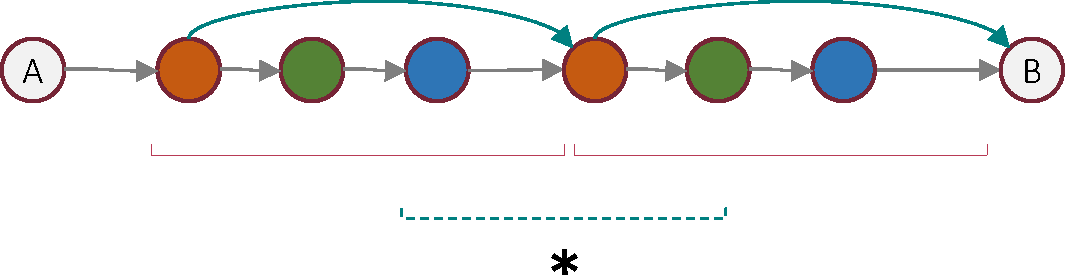
\includegraphics[width=\textwidth]{transitive-closure}
  \caption{Transitive Closure over Arbitrary Node Type and Edge Label Sequence}
  \label{fig:transitive-closure}
\end{figure}


\section{Control Flow Graph}

\section{Language Limitations}
